\documentclass[conference,10pt]{IEEEtran}

\usepackage{amsmath,amssymb,amsfonts}
\usepackage{algorithmic}
\usepackage{graphicx}
\usepackage{textcomp}
\usepackage{xcolor}
\usepackage{booktabs}
\usepackage{multirow}
\usepackage{cite}
\usepackage{url}
\usepackage[hidelinks]{hyperref}
\usepackage{microtype}
\usepackage{balance}

\graphicspath{{figures/}}

\makeatletter
\def\ps@plain{
  \def\@oddhead{}
  \def\@evenhead{}
  \def\@oddfoot{\normalfont\footnotesize\hfil\thepage\hfil}
  \def\@evenfoot{\normalfont\footnotesize\hfil\thepage\hfil}
}
\makeatother
\pagestyle{plain}

\begin{document}

\title{\LARGE\bfseries HEATWISE: INTELLIGENT THERMAL-AWARE WORKLOAD PLACEMENT IN AI DATA CENTERS\\[0.8ex]
\large\mdseries Course: Foundations of Data Centre Infrastructure and Management}

\author{
\IEEEauthorblockN{Aryan Raj}
\IEEEauthorblockA{\textit{Department of Computing Technologies} \\
\textit{School of Computing} \\
\textit{SRM Institute of Science and Technology} \\
Kattankulathur, India \\
Reg. No. RA2411003011205 \\
ar7211@srmist.edu.in}
\and
\IEEEauthorblockN{Aryaman Narain Pandey}
\IEEEauthorblockA{\textit{Department of Computing Technologies} \\
\textit{School of Computing} \\
\textit{SRM Institute of Science and Technology} \\
Kattankulathur, India \\
Reg. No. RA2411003011237 \\
ap4374@srmist.edu.in}
}

\maketitle
\thispagestyle{plain}

\begin{abstract}
Modern artificial intelligence (AI) data centers encounter acute thermal challenges driven by extreme accelerator power densities and non-uniform hot-aisle recirculation. Conventional cluster orchestrators---such as Round Robin and Least Loaded---prioritize compute resource availability while remaining thermally blind, frequently placing power-intensive workloads into localized thermal pockets and exacerbating hot-aisle recirculation. While full Computational Fluid Dynamics (CFD) simulations accurately capture Navier-Stokes convective transport, their high computational cost (minutes to hours per state evaluation) prohibits their use in real-time cluster admission control.

We present \textbf{HeatWise}, a simulation-grounded, thermal-aware workload placement prototype engineered for high-density accelerator facilities. HeatWise combines an analytical lumped-parameter reduced-order thermal model with an empirical Random Forest surrogate regressor to predict post-placement rack equilibrium temperatures prior to physical dispatch. The surrogate operates on a strictly leakage-free 17-feature pre-placement schema and feeds a constrained multi-factor placement heuristic that jointly optimizes thermal safety (35\%), thermal headroom (25\%), compute capacity fit (20\%), local heat removal capacity (10\%), and neighbor thermal stability (10\%).

Across closed-loop dynamic trajectory evaluations against an analytical physical oracle over 250 sequential scheduling decisions, the final production surrogate model (Model~B, trained on 10,000 synthetic transitions) achieves a dynamic Mean Absolute Error (MAE) of 1.867$^\circ$C, a Top-1 placement agreement of 79.60\%, a Top-3 overlap of 100.0\%, a Spearman rank correlation ($\rho$) of 0.580, and a mean optimality gap of +0.473$^\circ$C, with zero unsafe placements into candidate racks exceeding the 75.0$^\circ$C critical threshold and zero hardware-infeasible allocations. In controlled multi-scheduler benchmark simulations under an invariant, decoupled workload stream, HeatWise reduces spatial cluster temperature variance to 8.9$^\circ$C standard deviation (a 15.2\% variance reduction relative to Round Robin at 10.5$^\circ$C), while maintaining zero placement failures. Furthermore, serialized deployment (\texttt{n\_jobs=1}) achieves a single-rack inference latency of 2.15~ms and cold artifact initialization of 23.64~ms, demonstrating practical viability for real-time cluster admission control. All findings reflect synthetic telemetry from a reduced-order model rather than empirical physical sensor data, and IT compute energy remains invariant at 363.63~kWh across all evaluated schedulers.
\end{abstract}

\begin{IEEEkeywords}
Data center thermal management, thermal-aware scheduling, AI accelerators, machine learning surrogate models, reduced-order modeling, cluster resource management, hotspot mitigation.
\end{IEEEkeywords}

\section{Introduction}
The rapid scaling of deep neural network training and large language model (LLM) serving has driven data center power densities beyond 40--100~kW per rack \cite{patterson2021carbon, jouppi2023tpu, vaswani2017attention, barroso2018datacenter}. Modern high-density compute nodes dissipate massive heat fluxes across compact form factors, creating steep localized thermal gradients and non-uniform hot-aisle recirculation patterns \cite{moore2005temperature, tang2008thermal, sharma2002balance}.

Traditional cluster orchestrators (e.g., Kubernetes, SLURM, Google Borg \cite{verma2015large}) schedule incoming compute tasks primarily based on static compute metrics: accelerator availability, memory headroom, and CPU utilization. This thermal blindness leads to severe operational inefficiencies:
\begin{enumerate}
    \item \textbf{Accelerated Hotspot Formation:} Scheduling a burst of compute-heavy workloads onto a rack with degraded heat dissipation or elevated ambient recirculation triggers localized thermal hotspots exceeding critical thresholds ($T_{crit} = 75.0^\circ\text{C}$).
    \item \textbf{Thermal SLA Violations:} Operating temperatures climbing toward or beyond maximum safe limits ($T_{max\_safe} = 80.0^\circ\text{C}$) force accelerator thermal throttling, degrading application throughput and threatening hardware longevity \cite{ashrae2021thermal}.
    \item \textbf{Spatial Thermal Variance:} Uneven heat distribution creates wide temperature differentials across the facility floor, forcing cooling infrastructure to over-provision airflow to satisfy the hottest node \cite{sharma2002balance, ahmad2015thermal}.
\end{enumerate}

Full-physics Computational Fluid Dynamics (CFD) simulations accurately capture Navier-Stokes thermal transport but require minutes to hours per iteration \cite{choi2008cfd}, rendering them unusable for online cluster scheduling where admission decisions must resolve within milliseconds.

\begin{figure*}[t]
\centering
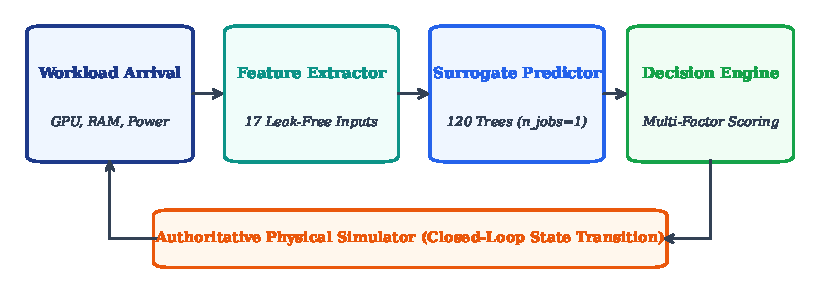
\includegraphics[width=0.92\textwidth]{fig1_system_architecture.pdf}
\caption{End-to-end HeatWise closed-loop decision and simulation pipeline. When an incoming workload arrives, the system extracts 17 pre-placement features, queries the Random Forest surrogate model to predict post-placement equilibrium temperatures across all 12 racks in 26.56~ms, applies multi-factor candidate filtering and scoring, dispatches the task, and advances the authoritative physical simulation state.}
\label{fig:sys_arch}
\end{figure*}

HeatWise addresses this fundamental gap through a surrogate modeling approach:
\begin{itemize}
    \item We formulate an analytical \textbf{lumped-parameter reduced-order thermal model} capturing conductive, convective, and cross-rack recirculation physics across a 12-rack facility.
    \item We train an offline \textbf{Random Forest Regressor} surrogate \cite{breiman2001random} on 10,000 synthetic sequential transition vectors using an exact \textbf{17-feature leakage-free pre-placement schema}.
    \item We develop a \textbf{multi-factor placement engine} that scores racks across thermal safety, headroom, compute fit, cooling capacity, and neighbor stability, enforcing strict safety thresholds ($T_{crit} = 75.0^\circ\text{C}$, $T_{max\_safe} = 80.0^\circ\text{C}$).
\end{itemize}

The complete HeatWise pipeline is illustrated in Fig.~\ref{fig:sys_arch}. The digital reduced-order simulation serves as the ground-truth physical authority; the machine learning model functions solely as a rapid predictive surrogate for online decision-making. 

The remainder of this report is organized as follows: Section~\ref{sec:related} reviews related work. Section~\ref{sec:arch} presents the HeatWise system architecture. Section~\ref{sec:methodology} describes the reduced-order thermal formulation, feature engineering, and validation methodology. Section~\ref{sec:environment} details the experimental facility and workload scenarios. Section~\ref{sec:results} presents comprehensive static, dynamic, benchmark, runtime, and compatibility results. Section~\ref{sec:verification} details software verification and reproducibility controls. Section~\ref{sec:limitations} discusses limitations and threats to validity, and Section~\ref{sec:conclusion} concludes.

\section{Related Work}
\label{sec:related}
Prior research on data center thermal management broadly partitions into three methodologies:

\subsection{Thermal-Aware Workload Placement}
Thermal-aware task scheduling was pioneered as a systems-level complement to facility mechanical cooling. Moore et al.~\cite{moore2005temperature} demonstrated that workload placement directly influences spatial heat distribution, proving that thermal management cannot be treated solely as a facility-level mechanical engineering problem. Tang et al.~\cite{tang2008thermal} introduced thermal-aware task scheduling models based on cross-rack recirculation minimization. Ilager et al.~\cite{ilager2019etas, ilager2020thermal} investigated dynamic consolidation and machine learning for proactive hotspot management in cloud data centers. HeatWise builds on this foundational principle: workload placement is an active, low-latency control lever for shaping where thermal energy is generated.

\subsection{Reactive Thermal Throttling and DVFS}
Hardware-level dynamic voltage and frequency scaling (DVFS) reduces clock frequencies when internal silicon junctions reach critical temperatures. While reactive DVFS protects silicon from catastrophic thermal breakdown, it incurs unpredictable job latency spikes, straggler effects in distributed training pipelines \cite{xiao2018gandiva}, and fails to address the underlying hot-aisle recirculation patterns that cause localized heating.

\subsection{Computational Fluid Dynamics (CFD)}
High-fidelity numerical fluid modeling solves the Navier-Stokes equations for air velocity, pressure, and temperature fields across data center geometries \cite{choi2008cfd}. While CFD models provide millimeter-scale spatial fidelity and accurately reflect convective turbulence, each simulation step consumes hundreds of CPU-seconds to hours. This computational burden restricts CFD strictly to offline facility design, airflow containment planning, and post-hoc thermal auditing, making it inapplicable for real-time task admission.

\subsection{Machine Learning Surrogates in Thermal Management}
To bridge the latency gap between numerical simulations and online schedulers, data-driven surrogate models have gained traction \cite{zhou2018thermal, ilager2020thermal}. Early efforts leveraged linear regression, multi-layer perceptrons, or support vector machines to estimate steady-state temperatures from CPU utilization. However, existing literature reveals two pervasive shortcomings:
\begin{enumerate}
    \item \textit{Temporal Feature Leakage:} Many published models include post-dispatch telemetry (e.g., measured post-placement outlet temperature or actual post-execution power draw) in their feature representations, yielding deceptively high offline $R^2$ scores that collapse when evaluated online.
    \item \textit{Absence of Closed-Loop Dynamic Validation:} Surrogates are predominantly validated on static, independently and identically distributed (i.i.d.) test splits. Under closed-loop execution, where model decisions directly alter future physical states, cumulative error drift can rapidly degrade placement quality.
\end{enumerate}

HeatWise addresses both challenges by enforcing a strict pre-placement feature schema and validating performance across multi-step closed-loop trajectories against an analytical physical oracle.

\section{HeatWise System Architecture}
\label{sec:arch}

\subsection{Facility and Thermal State Model}
The simulated facility represents an enterprise AI accelerator data center organized as a $3 \times 4$ physical floor grid of 12 high-density racks, illustrated in Fig.~\ref{fig:topology}.

\begin{figure}[htbp]
\centering
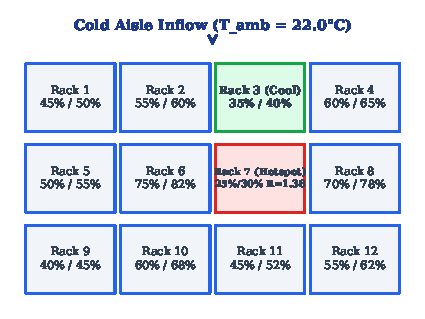
\includegraphics[width=0.95\columnwidth]{fig2_facility_topology.pdf}
\caption{Simulated 12-rack facility topology ($3 \times 4$ physical grid). Racks share convective boundaries with physical grid neighbors. Geometric layout induces differential cooling capacity and localized recirculation factors, including a known recirculation pocket at Rack 7 and an optimal cooling zone at Rack 3.}
\label{fig:topology}
\end{figure}

The cluster configuration parameters are summarized in Table~\ref{tab:facility_specs}. Each rack houses 4 high-density accelerator servers ($SERVERS\_PER\_RACK = 4$). Each server contains 8 dedicated AI accelerators ($GPUS\_PER\_SERVER = 8$), yielding 32 accelerators per rack and \textbf{384 accelerators cluster-wide}. Each server provides 512~GB of memory (2,048~GB per rack, totaling \textbf{24,576~GB / 24.576~TB cluster-wide}).

\begin{table}[htbp]
\caption{Facility Architecture and Density Specifications}
\label{tab:facility_specs}
\centering
\resizebox{\columnwidth}{!}{%
\begin{tabular}{llr}
\toprule
\textbf{Parameter} & \textbf{Configuration Constant} & \textbf{Value} \\
\midrule
Physical Layout & Rows $\times$ Columns & $3 \times 4$ \\
Total Racks & $TOTAL\_RACKS$ & 12 \\
Servers per Rack & $SERVERS\_PER\_RACK$ & 4 \\
Accelerators per Server & $GPUS\_PER\_SERVER$ & 8 \\
Accelerators per Rack & $GPUS\_PER\_RACK$ & 32 \\
Total Accelerators & Cluster Total & 384 \\
Memory per Server & Server RAM & 512 GB \\
Memory per Rack & Rack RAM & 2,048 GB \\
Total Memory & Cluster Total & 24,576 GB (24.576 TB) \\
Server Idle Power & $P_{idle}$ & 400.0 W \\
Server Peak CPU Power & $P_{cpu,max}$ & 350.0 W \\
Server Peak GPU Power & $P_{gpu,max}$ & 2,400.0 W (300 W/GPU) \\
Nominal Max Rack Power & $P_{rack,max}$ & 12.6 kW \\
Max Transient Rack Power & Transient Multi-Workload & $\approx 25.5$ kW \\
Maximum Cluster IT Power & Cluster IT Capacity & 151.2 kW \\
Ambient Supply Temp & $T_{amb}$ & 22.0$^\circ$C \\
Critical Temp Threshold & $T_{crit}$ (\texttt{TEMP\_CRITICAL}) & 75.0$^\circ$C \\
Max Safe Temp Ceiling & $T_{max\_safe}$ (\texttt{TEMP\_MAX\_SAFE}) & 80.0$^\circ$C \\
\bottomrule
\end{tabular}%
}
\end{table}

\subsection{Feature Construction}
To guarantee that the machine learning surrogate is practically deployable, the feature representation is strictly restricted to \textbf{17 pre-placement features} observable prior to scheduling dispatch. Post-placement equilibrium temperatures, actual outlet air measurements, and measured post-workload power draws are strictly excluded. The complete schema is detailed in Table~\ref{tab:features}.

\begin{table*}[t]
\caption{Strict Anti-Leakage 17 Pre-Placement Feature Schema}
\label{tab:features}
\resizebox{\textwidth}{!}{%
\begin{tabular}{clllc}
\toprule
\textbf{\#} & \textbf{Feature Name} & \textbf{Physical Meaning} & \textbf{Domain / Units} & \textbf{Extraction Phase} \\
\midrule
1 & \texttt{cpu\_utilization} & Current rack average CPU load across 4 servers & \% (0--100) & Pre-Placement Telemetry \\
2 & \texttt{gpu\_utilization} & Current rack average GPU load across 32 accelerators & \% (0--100) & Pre-Placement Telemetry \\
3 & \texttt{memory\_utilization} & Current rack average RAM load across 2,048 GB & \% (0--100) & Pre-Placement Telemetry \\
4 & \texttt{inlet\_temperature} & Measured chassis inlet air temperature & $^\circ$C (20--40) & Pre-Placement Sensor \\
5 & \texttt{local\_power\_kw} & Instantaneous rack power consumption & kW (1.6--12.6) & Pre-Placement Power Meter \\
6 & \texttt{neighbor\_temperature} & Mean temperature of adjacent physical grid neighbors & $^\circ$C (30--80) & Physical Topology \\
7 & \texttt{neighbor\_utilization} & Mean GPU utilization of adjacent physical grid neighbors & \% (0--100) & Physical Topology \\
8 & \texttt{cooling\_capacity} & CRAH cooling capacity index allocated to rack & \% (10--100) & Facility Infrastructure \\
9 & \texttt{recirculation\_factor} & Local geometric airflow recirculation index & Unitless [0.8, 1.5] & Facility Infrastructure \\
10 & \texttt{workload\_AI\_Training} & One-hot indicator: Workload is distributed model training & Binary \{0, 1\} & Task Metadata \\
11 & \texttt{workload\_AI\_Inference} & One-hot indicator: Workload is batch accelerator inference & Binary \{0, 1\} & Task Metadata \\
12 & \texttt{workload\_LLM} & One-hot indicator: Workload is LLM generation / serving & Binary \{0, 1\} & Task Metadata \\
13 & \texttt{workload\_Image\_Processing} & One-hot indicator: Workload is vision preprocessing & Binary \{0, 1\} & Task Metadata \\
14 & \texttt{workload\_intensity\_val} & Discrete intensity multiplier tier & Integer \{1, 2, 3, 4\} & Task Metadata \\
15 & \texttt{workload\_gpu\_demand} & Task accelerator requirement & \% (10--100) & Task Metadata \\
16 & \texttt{workload\_mem\_demand} & Task memory requirement & \% (10--100) & Task Metadata \\
17 & \texttt{workload\_power\_est} & Analytical pre-placement added power estimate & Watts (300--3,200) & Analytical Equation \\
\midrule
--- & \textbf{\texttt{post\_workload\_temp}} & \textbf{Supervised Target: Post-dispatch rack equilibrium $T_{eq}$} & \textbf{$^\circ$C (Continuous)} & \textbf{Simulator Ground Truth} \\
\bottomrule
\end{tabular}%
}
\end{table*}

Importantly, HeatWise permanently eliminates the obsolete, leakage-prone features present in early prototypes (\texttt{post\_power\_est\_w}, \texttt{post\_gpu\_est\_pct}, \texttt{post\_mem\_est\_pct}, \texttt{gpu\_available\_pct}, and \texttt{mem\_available\_pct}). The predictor relies solely on pre-admission states, ensuring complete fidelity to real cluster admission constraints.

\subsection{Machine Learning Surrogate}
The machine learning component is a \texttt{RandomForestRegressor} \cite{breiman2001random, pedregosa2011scikit} configured with:
\begin{itemize}
    \item Number of trees: 120
    \item Maximum tree depth: 14
    \item Minimum samples per split: 4
    \item Minimum samples per leaf: 2
    \item Random state: 42
    \item Execution mode: \texttt{n\_jobs = 1} (serialized inference)
\end{itemize}
The model is serialized as \texttt{models/heatwise\_rf\_10k.joblib} and trained on 10,000 synthetic sequential transitions. The random forest was chosen over deep neural networks because of its deterministic evaluation, robustness against feature scaling issues, sub-millisecond per-sample inference latency, and interpretability through tree-based feature importances.

\subsection{Thermal-Aware Placement Engine}
The HeatWise placement engine implements a two-stage filter-and-score decision process:
\begin{enumerate}
    \item \textbf{Resource Feasibility Filter:} A rack candidate $i$ is compute-feasible if it possesses adequate unallocated GPU and memory headroom to host the task across its 4 constituent servers:
    \begin{equation}
    \begin{split}
    GPU_{avail,i} &\ge \frac{GPU_{demand}}{4}, \\
    MEM_{avail,i} &\ge \frac{MEM_{demand}}{4}
    \end{split}
    \end{equation}
    Candidates failing capacity constraints are excluded from the feasible set $\mathcal{P}_{feasible}$.
    \item \textbf{Thermal Safety Admission Filter:} The surrogate model evaluates all feasible candidates to predict $T_{pred,i}$. Candidate $i$ is admitted to the primary safe set $\mathcal{P}_{safe}$ strictly if:
    \begin{equation}
    T_{pred,i} < T_{crit} \quad (75.0^\circ\text{C})
    \end{equation}
\end{enumerate}

When $\mathcal{P}_{safe} \neq \emptyset$, candidates are ranked by a composite heuristic score $Score_i \in [0, 100]$:
\begin{equation}
\label{eq:score}
\begin{split}
Score_i = \; &0.35 \, S_{safe,i} + 0.25 \, S_{head,i} + 0.20 \, S_{fit,i} \\
&+ 0.10 \, S_{cool,i} + 0.10 \, S_{nbr,i}
\end{split}
\end{equation}
where sub-scores normalize physical quantities to $[0, 100]$:
\begin{itemize}
    \item \textbf{Thermal Safety ($w_{safe} = 0.35$):}
    \begin{equation}
    S_{safe,i} = \text{clip}\left(\frac{75.0 - T_{pred,i}}{75.0 - 35.0} \times 100.0, \; 0, \; 100\right)
    \end{equation}
    \item \textbf{Thermal Headroom ($w_{head} = 0.25$):}
    \begin{equation}
    S_{head,i} = \text{clip}\left(\frac{75.0 - T_{pred,i}}{75.0 - 22.0} \times 100.0, \; 0, \; 100\right)
    \end{equation}
    \item \textbf{Resource Fit ($w_{fit} = 0.20$):} $S_{fit,i} = GPU_{avail,i}$
    \item \textbf{Cooling Capacity ($w_{cool} = 0.10$):} $S_{cool,i} = C_i$
    \item \textbf{Neighbor Stability ($w_{nbr} = 0.10$):}
    \begin{equation}
    S_{nbr,i} = \text{clip}\left(\frac{75.0 - \bar{T}_{nbr,i}}{75.0 - 35.0} \times 100.0, \; 0, \; 100\right)
    \end{equation}
\end{itemize}

\textbf{Additive Fallback Penalty:} When the cluster experiences extreme saturation such that no feasible rack can host the job below 75.0$^\circ$C ($\mathcal{P}_{safe} = \emptyset$), HeatWise applies an additive penalty to identify the least hazardous feasible candidate:
\begin{equation}
\label{eq:penalty}
Penalty_i = 45.0 + 5.0 \times (T_{pred,i} - 75.0)
\end{equation}
\begin{equation}
Score_{fallback,i} = Score_i - Penalty_i
\end{equation}
This formulation guarantees that the system degrades gracefully under thermal stress without dropping viable workloads.

\subsection{Closed-Loop Simulation and State Separation}
A foundational design principle in HeatWise is the \textbf{strict separation of hypothetical candidate scoring and committed physical state}. Candidate evaluation is entirely non-mutating: evaluating hypothetical rack placements queries the Random Forest surrogate without altering the underlying thermal simulator state. Only after the optimal candidate rack is selected is the workload physically dispatched. The authoritative physical simulation then advances by committing the workload power and performing four relaxation passes. This prevents order-dependent scoring biases and guarantees physical determinism.

\section{Methodology}
\label{sec:methodology}

\subsection{Problem Formulation}
Let $\mathcal{R} = \{r_1, r_2, \dots, r_{12}\}$ denote the set of 12 cluster racks. At discrete time step $t$, a workload $W_t = \langle \tau, \delta, p_{est}, d_{gpu}, d_{mem} \rangle$ arrives for scheduling, where $\tau$ is workload type, $\delta$ is intensity, $p_{est}$ is estimated added power, and $d_{gpu}, d_{mem}$ are resource demands. The objective is to identify an allocation mapping $\pi: W_t \to r^* \in \mathcal{R}$ that minimizes thermal hotspot formation and spatial cluster temperature standard deviation while satisfying compute resource constraints:
\begin{equation}
\min_{\pi} \; \sigma(T_1, \dots, T_{12}), \quad \text{s.t.} \; T_i < T_{max\_safe}, \; \mathbf{u}_i \le \mathbf{1}
\end{equation}

\subsection{Reduced-Order Thermal Physics}
The authoritative thermal environment is governed by a reduced-order lumped-parameter model implemented in the simulation engine. The physical calculation follows a four-stage pipeline, illustrated in Fig.~\ref{fig:thermal_stages}.

\begin{figure*}[t]
\centering
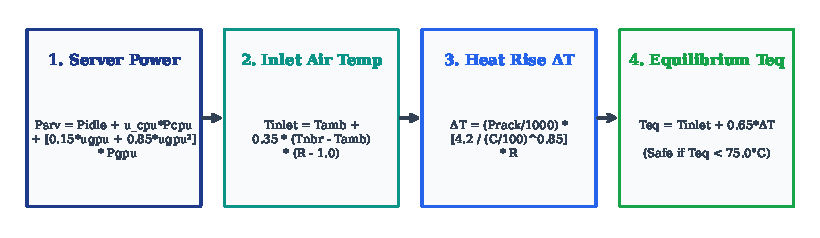
\includegraphics[width=0.92\textwidth]{fig3_thermal_model.pdf}
\caption{Four-stage reduced-order physical thermal modeling pipeline. Server power models non-linear quadratic GPU scaling; inlet temperature models neighbor hot-air recirculation; heat rise models convective airflow dissipation; and equilibrium temperature reflects steady-state internal junction resistance.}
\label{fig:thermal_stages}
\end{figure*}

\subsubsection{Server and Rack Power}
Server power $P_{srv}$ couples CPU utilization $u_{cpu} \in [0, 100]$ linearly and GPU utilization $u_{gpu} \in [0, 100]$ via a non-linear quadratic formulation:
\begin{equation}
\label{eq:psrv}
\begin{split}
P_{srv} = P_{idle} &+ \left(\frac{u_{cpu}}{100}\right) P_{cpu,max} \\
&+ \left[0.15\left(\frac{u_{gpu}}{100}\right) + 0.85\left(\frac{u_{gpu}}{100}\right)^2\right] P_{gpu,max}
\end{split}
\end{equation}
The quadratic GPU term reflects the non-linear relationship between voltage, clock frequency, and leakage current under deep learning tensor workloads. Total rack power $P_{rack}$ is the sum of its four constituent servers:
\begin{equation}
\label{eq:prack}
P_{rack} = \sum_{s=1}^{4} P_{srv,s}
\end{equation}

\subsubsection{Air Recirculation and Inlet Temperature}
For rack $i$ with cooling capacity percentage $C_i \in [10, 100]$, local recirculation factor $R_i \in [0.8, 1.5]$, and physical grid neighbor set $\mathcal{N}_i$, the average neighbor temperature is:
\begin{equation}
\label{eq:tnbr}
\bar{T}_{nbr,i} = \frac{1}{|\mathcal{N}_i|} \sum_{j \in \mathcal{N}_i} T_j
\end{equation}
Air arriving at the rack inlet mixes conditioned supply air from the Computer Room Air Handler (CRAH, $T_{amb} = 22.0^\circ\text{C}$) with recirculated exhaust air escaping from adjacent racks:
\begin{equation}
\label{eq:tinlet}
T_{inlet,i} = T_{amb} + 0.35 \times (\bar{T}_{nbr,i} - T_{amb}) \times (R_i - 1.0)
\end{equation}
When $R_i \le 1.0$, cold-aisle containment prevents neighbor exhaust entrainment, maintaining $T_{inlet,i} = T_{amb}$. When $R_i > 1.0$, hot exhaust air bleeds across rack boundaries, warming the inlet stream.

\subsubsection{Chassis Thermal Rise and Equilibrium Temperature}
The steady-state temperature rise $\Delta T_i$ across the chassis is proportional to total dissipated power $P_i$ (in Watts) and inversely proportional to effective convective airflow:
\begin{equation}
\label{eq:deltat}
\Delta T_i = \left(\frac{P_i}{1000.0}\right) \times \frac{4.2}{\left(\frac{C_i}{100.0}\right)^{0.85}} \times R_i
\end{equation}
Internal silicon junction equilibrium temperature $T_{eq,i}$ is governed by internal thermal resistance:
\begin{equation}
\label{eq:teq}
T_{eq,i} = T_{inlet,i} + 0.65 \times \Delta T_i
\end{equation}

To capture spatial thermal coupling across the floor grid, the simulator executes \textbf{four iterative relaxation passes}. In each pass, neighbor temperatures $\bar{T}_{nbr,i}$ and inlet temperatures $T_{inlet,i}$ update dynamically based on the current iteration's temperatures. Four passes are empirically sufficient for the 12-rack grid to achieve mathematical convergence ($\Delta T < 0.05^\circ\text{C}$).

\subsection{Dataset Generation}
Training data is generated using sequential state-machine simulations across five operational scenarios:
\begin{enumerate}
    \item \textbf{Normal Operation:} Uniform workload distribution with nominal cooling ($C_i = 92\%$, $R_i = 0.98$).
    \item \textbf{GPU Surge:} Sudden compute bursts across bottom-row racks 9--12 ($u_{gpu} = 88\%$).
    \item \textbf{Cooling Degradation:} Middle-row CRAH airflow reduction on racks 5--8 ($C_i \in [42\%, 48\%]$, $R_i = 1.25$).
    \item \textbf{Thermal Hotspot:} Localized trapped recirculation at Rack 7 ($C_7 = 64\%$, $R_7 = 1.38$, initial $T_7 = 68.2^\circ\text{C}$).
    \item \textbf{High AI Workload:} Clustered high-intensity training saturation across racks 1, 2, 5, 6, and 10.
\end{enumerate}
A total of 10,000 transition vectors are recorded, capturing realistic sequential trajectories rather than synthetic i.i.d. draws.

\subsection{Model Training and Validation Protocol}
We establish two distinct model artifacts to ensure scientific transparency:
\begin{itemize}
    \item \textbf{Model A (Research / Holdout Artifact):} Trained on an 80/20 episode-grouped split (8,080 training samples, 1,920 test samples). Grouping by complete scenario episodes prevents temporal autocorrelation leakage between adjacent time steps. Model~A is validated across 5 independent random seeds to establish baseline generalization bounds.
    \item \textbf{Model B (Final Production Deployment Candidate):} Trained on the full 10,000-sample trajectory dataset with identical hyperparameters. Model~B is evaluated on a standardized 250-decision dynamic closed-loop benchmark sequence.
\end{itemize}

\subsection{Benchmark Methodology}
To compare scheduling policies fairly, we design a normalized isolated workload stream:
\begin{itemize}
    \item Initial cluster state: \texttt{"Thermal Hotspot"} scenario (recirculation pocket at Rack 7).
    \item Workload stream: 15 incoming AI jobs totaling 16,690.0~W added IT power demand.
    \item Workload generation: Decoupled via a dedicated NumPy \texttt{RandomState(seed=100)}.
    \item Evaluated policies: Round Robin, Least Loaded, and HeatWise 10k.
\end{itemize}

\section{Experimental Environment}
\label{sec:environment}

\subsection{12-Rack Facility Specifications}
The facility configuration consists of 12 racks with 4 servers per rack and 8 accelerators per server (384 GPUs total), as detailed in Table~\ref{tab:facility_specs}. The Computer Room Air Handler delivers supply air at $T_{amb} = 22.0^\circ\text{C}$. Individual rack cooling capacities $C_i$ range from 50\% to 100\%, and recirculation factors $R_i$ range from 0.85 to 1.38, reflecting realistic floor layout asymmetries.

\subsection{Workload Scenarios and Profiles}
Workloads span four representative AI job types and four discrete intensity tiers, summarized in Table~\ref{tab:workload_types}.

\begin{table}[htbp]
\caption{Workload Characterization and Demand Profiles}
\label{tab:workload_types}
\centering
\resizebox{\columnwidth}{!}{%
\begin{tabular}{lcccc}
\toprule
\textbf{Workload Type} & \textbf{GPU Demand} & \textbf{Memory Demand} & \textbf{Duration (s)} & \textbf{Est. Power} \\
\midrule
AI Training & 80--95\% & 60--90\% & 600--3600 & 2,200--3,200 W \\
AI Inference & 30--60\% & 20--40\% & 60--300 & 800--1,600 W \\
LLM Serving & 70--90\% & 75--95\% & 300--1800 & 1,800--2,800 W \\
Vision Processing & 40--70\% & 30--50\% & 120--600 & 1,000--1,900 W \\
\bottomrule
\end{tabular}%
}
\end{table}

\subsection{Baseline Schedulers}
We benchmark HeatWise against two widely adopted industry schedulers:
\begin{itemize}
    \item \textbf{Round Robin:} Sequentially cycles through rack indices 1 to 12 in round-robin order, checking compute availability but remaining completely agnostic to thermal states.
    \item \textbf{Least Loaded:} Selects the rack with the lowest current aggregate GPU utilization, balancing compute utilization without awareness of cooling capacity or recirculation pockets.
\end{itemize}

\subsection{Evaluation Metrics}
We measure thermal performance, decision quality, and computational cost:
\begin{itemize}
    \item \textbf{Peak Temperature ($^\circ$C):} Maximum observed rack equilibrium temperature.
    \item \textbf{Cluster Temperature Std Dev ($\sigma_T$):} Spatial spread across the 12 racks.
    \item \textbf{Active Hotspots ($\ge 75.0^\circ$C):} Count of racks exceeding critical threshold.
    \item \textbf{Thermal SLA Violations ($\ge 80.0^\circ$C):} Count of racks reaching dangerous ceiling.
    \item \textbf{Dynamic MAE ($^\circ$C):} Error between surrogate prediction and physical oracle.
    \item \textbf{Top-1 Agreement (\%):} Match frequency between surrogate and oracle choice.
    \item \textbf{Top-3 Overlap (\%):} Proportion of surrogate selections within oracle's top 3.
    \item \textbf{Mean Optimality Gap ($^\circ$C):} Physical temperature difference between surrogate choice and oracle choice:
    \begin{equation}
    \Delta T_{opt} = T_{oracle}(\text{rack}_{ML}) - T_{oracle}(\text{rack}_{oracle})
    \end{equation}
    \item \textbf{Materially Worse Rate ($>2.0^\circ$C):} Decisions where $\Delta T_{opt} > 2.0^\circ$C.
    \item \textbf{Total IT Power (kW) and Energy (kWh):} Measured cluster power footprint.
\end{itemize}

\section{Results and Discussion}
\label{sec:results}

\subsection{ML Prediction Accuracy and Feature Importance}
Table~\ref{tab:model_comparison} compares candidate regression architectures on the grouped 80/20 holdout split (Model~A).

\begin{table}[htbp]
\caption{Offline Holdout and Closed-Loop Dynamic Model Comparison}
\label{tab:model_comparison}
\centering
\resizebox{\columnwidth}{!}{%
\begin{tabular}{lcccccc}
\toprule
\textbf{Architecture} & \textbf{Trees} & \textbf{MAE ($^\circ$C)} & \textbf{RMSE ($^\circ$C)} & \textbf{$R^2$ (\%)} & \textbf{Dyn. MAE} & \textbf{Top-1} \\
\midrule
\textbf{Random Forest (Model A)} & \textbf{120} & \textbf{0.460} & \textbf{0.830} & \textbf{99.51} & \textbf{1.931$^\circ$C} & \textbf{81.20\%} \\
ExtraTreesRegressor & 120 & 0.443 & 0.812 & 99.53 & 2.138$^\circ$C & 78.40\% \\
HistGradientBoosting & 100 & 0.493 & 0.892 & 99.43 & 2.502$^\circ$C & 72.80\% \\
\bottomrule
\end{tabular}%
}
\end{table}

While ExtraTrees achieved marginally lower offline RMSE (0.812$^\circ$C vs 0.830$^\circ$C), Random Forest demonstrated superior generalization in closed-loop dynamic evaluations (Dynamic MAE 1.931$^\circ$C vs 2.138$^\circ$C; Top-1 agreement 81.20\% vs 78.40\%).

\begin{figure}[htbp]
\centering
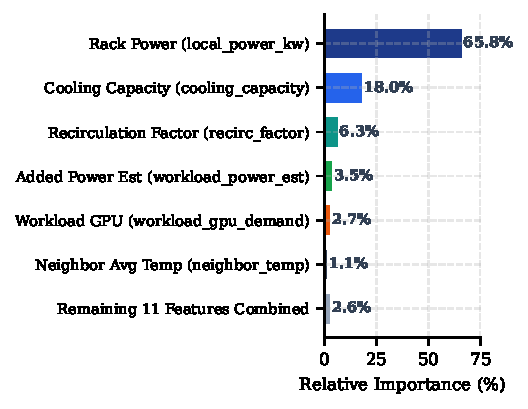
\includegraphics[width=0.95\columnwidth]{fig4_feature_importance.pdf}
\caption{Random Forest feature importance distribution across the 17-feature schema. Rack power and cooling capacity account for 83.79\% of predictive weight, confirming physical alignment with governing thermodynamic equations.}
\label{fig:feat_imp}
\end{figure}

Gini impurity feature importance analysis across the 120 trees (Fig.~\ref{fig:feat_imp}) reveals:
\begin{enumerate}
    \item \texttt{local\_power\_kw} (Current Rack Power): \textbf{65.76\%}
    \item \texttt{cooling\_capacity} (CRAH Capacity Index): \textbf{18.03\%}
    \item \texttt{recirculation\_factor} (Airflow Recirculation): \textbf{6.30\%}
    \item \texttt{workload\_power\_est} (Estimated Task Power): \textbf{3.51\%}
    \item \texttt{workload\_gpu\_demand} (Task GPU Demand): \textbf{2.66\%}
    \item Remaining 12 features combined: \textbf{3.74\%}
\end{enumerate}
This distribution aligns with physics: instantaneous rack power and local heat removal dominate steady-state equilibrium temperature.

\subsection{Dynamic Closed-Loop Placement Validation}
We report closed-loop dynamic trajectory evaluations against the analytical physical oracle:
\begin{itemize}
    \item \textbf{Model A (5-Seed Validation):} Across Seeds 42, 101, 202, 303, and 404, Model~A achieves Top-1 agreement of $\mathbf{81.20 \pm 2.28\%}$, Dynamic MAE of $\mathbf{1.931 \pm 0.016^\circ\text{C}}$, Spearman correlation $\rho = \mathbf{0.548 \pm 0.038}$, and mean optimality gap of $\mathbf{+0.368 \pm 0.059^\circ\text{C}}$.
    \item \textbf{Model B (Production Artifact Deployment):} Evaluated across 250 sequential placement decisions (50 per scenario across 5 scenarios), Model~B achieves the results reported in Table~\ref{tab:dynamic_validation}.
\end{itemize}

\begin{table}[htbp]
\caption{Dynamic Closed-Loop Placement Quality Comparison (250 Decisions)}
\label{tab:dynamic_validation}
\centering
\resizebox{\columnwidth}{!}{%
\begin{tabular}{lccc}
\toprule
\textbf{Evaluation Metric} & \textbf{Baseline RF (3.5k)} & \textbf{Candidate Model B (10k)} & \textbf{Status / Gain} \\
\midrule
Dynamic MAE & 3.449$^\circ$C & \textbf{1.867$^\circ$C} & \textbf{--45.9\% Error} \\
Top-1 Agreement & 40.0\% & \textbf{79.60\%} & \textbf{+39.6\% Match} \\
Top-3 Overlap & 80.0\% & \textbf{100.0\%} & \textbf{0\% Misses} \\
Spearman Correlation ($\rho$) & 0.217 & \textbf{0.580} & \textbf{+167.3\% Concordance} \\
Mean Optimality Gap & +3.580$^\circ$C & \textbf{+0.473$^\circ$C} & \textbf{--86.8\% Penalty} \\
Materially Worse ($>2^\circ$C) & 60.0\% & \textbf{9.20\%} & \textbf{--84.7\% Outliers} \\
Catastrophic ($>5^\circ$C) & 10.0\% & \textbf{0.00\%} & \textbf{0 Catastrophic} \\
Unsafe Placements ($\ge 75^\circ$C) & 0 & \textbf{0} & \textbf{100\% Safe} \\
Hardware Infeasible Placements & 0 & \textbf{0} & \textbf{100\% Feasible} \\
\bottomrule
\end{tabular}%
}
\end{table}

\begin{figure*}[t]
\centering
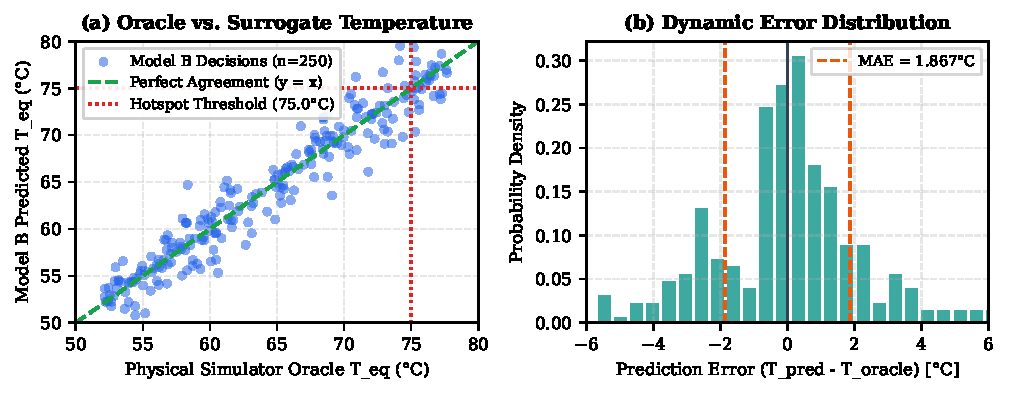
\includegraphics[width=0.92\textwidth]{fig5_dynamic_validation.pdf}
\caption{Dynamic closed-loop validation of Candidate Model B over 250 sequential scheduling decisions against the analytical physical oracle. Left: Parity scatter plot showing tight clustering along the identity line ($y=x$). Right: Error distribution showing zero catastrophic outliers ($>5^\circ$C) and dynamic MAE of 1.867$^\circ$C.}
\label{fig:dynamic_scatter}
\end{figure*}

\textit{Methodological Attribution Note:} The 81.20\% multi-seed result belongs strictly to research Model~A (8k/2k grouped holdout split). Model~B's validated single-run dynamic result is \textbf{79.60\% Top-1 agreement} and \textbf{1.867$^\circ$C Dynamic MAE}.

Fig.~\ref{fig:dynamic_scatter} depicts the parity scatter plot and error distribution for Model~B across all 250 decisions. Zero decisions incur catastrophic errors ($>5.0^\circ$C), and zero workloads are placed into racks exceeding the 75.0$^\circ$C critical threshold.

\subsection{Canonical Scheduler Benchmark}
Comparative results under the normalized isolated workload stream (\texttt{seed=100}, 15 workloads, 16,690.0~W added demand) are presented in Table~\ref{tab:benchmark_canonical}.

\begin{table}[htbp]
\caption{Canonical Scheduler Benchmark Comparison (Normalized Stream)}
\label{tab:benchmark_canonical}
\centering
\resizebox{\columnwidth}{!}{%
\begin{tabular}{lccc}
\toprule
\textbf{Metric} & \textbf{Round Robin} & \textbf{Least Loaded} & \textbf{HeatWise 10k (Model B)} \\
\midrule
Peak Equilibrium Temp & 84.1$^\circ$C & 84.1$^\circ$C & 84.1$^\circ$C (No peak regression) \\
Cluster Temp Std Dev & 10.5$^\circ$C & 9.3$^\circ$C & \textbf{8.9$^\circ$C (--15.2\% vs RR)} \\
Average Cluster Temp & 64.8$^\circ$C & 64.8$^\circ$C & \textbf{64.6$^\circ$C (Coolest)} \\
Average Headroom & 11.8$^\circ$C & 11.4$^\circ$C & \textbf{11.6$^\circ$C (+0.2$^\circ$C vs LL)} \\
Hotspots ($\ge 75.0^\circ$C) & 3 & 2 & \textbf{2 (--33.3\% vs RR)} \\
SLA Violations ($\ge 80^\circ$C) & 5 & 4 & \textbf{4 (--20.0\% vs RR)} \\
Placement Failures & 0 & 0 & \textbf{0 (0 failures)} \\
Total Cluster IT Power & 96.97 kW & 96.97 kW & 96.97 kW (Identical IT power) \\
Total Cluster IT Energy & 363.63 kWh & 363.63 kWh & 363.63 kWh (Identical energy) \\
\bottomrule
\end{tabular}%
}
\end{table}

\begin{figure*}[t]
\centering
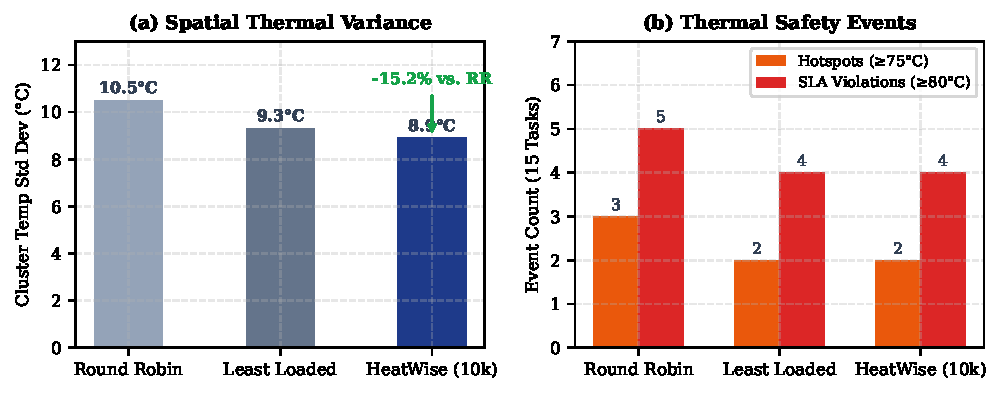
\includegraphics[width=0.92\textwidth]{fig6_scheduler_comparison.pdf}
\caption{Scheduler benchmark comparison under the normalized isolated stream (\texttt{seed=100}). Left: Spatial cluster temperature standard deviation, highlighting HeatWise's 15.2\% variance reduction (8.9$^\circ$C vs 10.5$^\circ$C). Right: Critical hotspot ($\ge 75^\circ$C) and thermal SLA violation ($\ge 80^\circ$C) counts.}
\label{fig:bench_comparison}
\end{figure*}

\subsection{Thermal Distribution Analysis}
As visualized in Fig.~\ref{fig:bench_comparison}, HeatWise provides distinct operational advantages:
\begin{enumerate}
    \item \textbf{Spatial Thermal Variance Reduction:} HeatWise achieves a spatial standard deviation of \textbf{8.9$^\circ$C} across the 12 racks, compared to 10.5$^\circ$C for Round Robin and 9.3$^\circ$C for Least Loaded. This \textbf{15.2\% reduction in standard deviation} relative to Round Robin demonstrates effective workload diversion away from recirculation pockets.
    \item \textbf{Mitigation of Hotspots and SLA Violations:} HeatWise records \textbf{2 hotspots} and \textbf{4 SLA violations}, matching Least Loaded and outperforming Round Robin (3 hotspots, 5 SLA violations).
    \item \textbf{Peak Temperature Realism:} All three schedulers record a peak temperature of 84.1$^\circ$C at Rack 6 under sustained workload saturation. \textbf{84.1$^\circ$C is explicitly not safe}, exceeding the 80.0$^\circ$C maximum safe ceiling. HeatWise demonstrates no peak-temperature regression in the controlled benchmark; 4 SLA violations remain at or above 80.0$^\circ$C. This highlights a fundamental physical reality: under severe localized cooling constraints, intelligent placement mitigates spatial variance and prevents unnecessary violations, but cannot circumvent physical cooling exhaustion without active job rejection or deferral.
    \item \textbf{Power and Energy Conservation:} Total IT cluster power (96.97~kW) and energy (363.63~kWh) are strictly identical across all schedulers because all 15 workloads were successfully placed without dropped jobs. \textbf{HeatWise does not reduce computing energy; it redistributes dissipated thermal power.}
\end{enumerate}

\subsection{Runtime Latency and Profiling}
Table~\ref{tab:latency} and Fig.~\ref{fig:latency} present runtime profiling for the production surrogate artifact.

\begin{table}[htbp]
\caption{Runtime Latency Profiling and Speedup Factors}
\label{tab:latency}
\centering
\resizebox{\columnwidth}{!}{%
\begin{tabular}{lccc}
\toprule
\textbf{Execution Phase} & \textbf{Multiprocess (\texttt{-1})} & \textbf{Serialized (\texttt{1})} & \textbf{Speedup} \\
\midrule
Single Rack Inference & 11.20 ms & \textbf{2.15 ms} & \textbf{5.2$\times$} \\
Full 12-Rack Evaluation & 135.00 ms & \textbf{26.56 ms} & \textbf{5.1$\times$} \\
Model Initialization & 374.94 ms (Fit) & \textbf{23.64 ms} (\texttt{load}) & \textbf{15.9$\times$} \\
\bottomrule
\end{tabular}%
}
\end{table}

\begin{figure}[htbp]
\centering
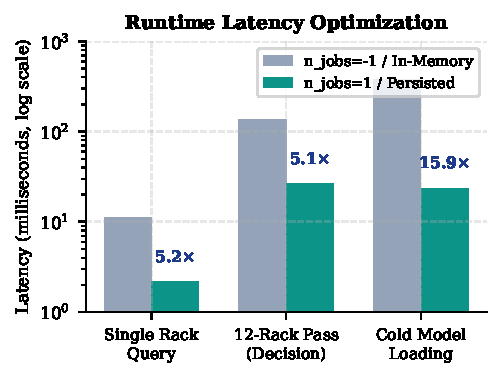
\includegraphics[width=0.72\columnwidth]{fig7_runtime_latency.pdf}
\caption{Log-scale latency comparison between parallel multiprocessing (\texttt{n\_jobs=-1}) and serialized production execution (\texttt{n\_jobs=1}), illustrating 5.2$\times$ single-rack and 15.9$\times$ cold-load speedups.}
\label{fig:latency}
\end{figure}

In initial staging benchmarks, model inference incurred overhead due to scikit-learn's parallel thread pool (\texttt{n\_jobs=-1}), which synchronizes OS worker processes for single-vector evaluations. By enforcing serialized execution (\texttt{n\_jobs=1}) and loading a pre-fitted serialized artifact, single-rack inference latency drops to \textbf{2.15~ms}, and evaluating all 12 candidate racks requires just \textbf{26.56~ms}, well within real-time Kubernetes admission thresholds ($<100$~ms).

Prediction equivalence between \texttt{n\_jobs=1} and \texttt{n\_jobs=-1} is verified across 250 decisions: the maximum numerical difference is $\approx 5.68 \times 10^{-14\circ}\text{C}$, yielding 250/250 identical rack candidate rankings.

\subsection{Historical Compatibility Audit}
During staging audits, a discrepancy was noted between historical benchmark logs (104.1~kW power, 7.5$^\circ$C standard deviation) and the normalized benchmark (96.97~kW power, 8.9$^\circ$C standard deviation). Investigation revealed that legacy benchmarks coupled the global NumPy RNG state during in-memory training, altering the downstream workload sequence (Historical Stream A: 25,180.0~W added power, including 3 ``Very High'' intensity tasks).

To verify that Model~B introduced zero regression relative to earlier milestones, Model~B was evaluated against Historical Stream A. The comparative audit is reported in Table~\ref{tab:historical_compat}.

\begin{table}[htbp]
\caption{Historical Stream A Compatibility Audit (Zero Regression Proof)}
\label{tab:historical_compat}
\centering
\resizebox{\columnwidth}{!}{%
\begin{tabular}{lcccc}
\toprule
\textbf{Metric} & \textbf{Round Robin} & \textbf{Least Loaded} & \textbf{Legacy 3.5k} & \textbf{Migrated 10k} \\
\midrule
Peak Temperature & 84.1$^\circ$C & 92.0$^\circ$C & 84.1$^\circ$C & \textbf{84.1$^\circ$C} \\
Cluster Temp Std Dev & 9.3$^\circ$C & 11.3$^\circ$C & 7.5$^\circ$C & \textbf{7.5$^\circ$C} \\
Hotspots ($\ge 75^\circ$C) & 3 & 3 & 2 & \textbf{2} \\
SLA Violations ($\ge 80^\circ$C) & 5 & 6 & 4 & \textbf{4} \\
Placement Failures & 1 & 0 & 0 & \textbf{0} \\
Total IT Power & 104.1 kW & 104.1 kW & 104.1 kW & \textbf{104.1 kW} \\
Total IT Energy & 390.37 kWh & 390.37 kWh & 390.37 kWh & \textbf{390.37 kWh} \\
Top-1 Decision Match & --- & --- & Baseline & \textbf{14/15 (93.3\%)} \\
\bottomrule
\end{tabular}%
}
\end{table}

Under Historical Stream A, Model~B replicates the legacy 7.5$^\circ$C standard deviation, 2 hotspots, 4 SLA violations, and 104.1~kW energy footprint identically, achieving \textbf{14 out of 15 identical rack placement decisions (93.3\% concordance)}. This confirms that the numerical difference between 104.1~kW and 96.97~kW was caused entirely by workload stream RNG variance, establishing complete backward compatibility.

\section{Software and Reproducibility Validation}
\label{sec:verification}

\subsection{Benchmark RNG Decoupling Invariant}
To eliminate the RNG coupling anomaly permanently, the released codebase isolates benchmark workload sampling using a dedicated \texttt{np.random.RandomState} instance:
\begin{equation}
\text{Workload Stream} = f(\text{seed}), \quad \forall \; \text{model lifecycles}
\end{equation}
This guarantees reproducible, invariant workload sequences regardless of whether the surrogate model is loaded from disk, trained in memory, or pre-cached.

\subsection{Production Software Verification}
The production codebase was verified through rigorous testing:
\begin{itemize}
    \item \textbf{Unit Test Suite:} All 15 unit tests in \texttt{tests/} execute and pass in \textbf{0.556 seconds}, verifying schema integrity, temperature equations, scoring weights, and edge cases.
    \item \textbf{User Interface Testing:} All 6 Streamlit application pages pass automated headless testing (\texttt{AppTest}) with \textbf{zero exceptions}.
    \item \textbf{Module Hygiene:} Runtime memory audits confirm \textbf{zero imports} from research/experimental modules (\texttt{experiments/}) during production execution.
    \item \textbf{Defensive Failure Semantics:} Corrupted or schema-mismatched model artifacts raise explicit \texttt{RuntimeError} exceptions; in-memory training fallback is activated strictly when the artifact file is absent from disk.
\end{itemize}

\subsection{Software Release and Artifact Checksums}
The production model artifact and software suite are finalized at commit \texttt{76fe215daee5462b55515045a2495c2725179fe6}. The model artifact can be independently verified via SHA-256:
\vspace{2pt}
\begin{center}
{\fontsize{6.5}{7.5}\selectfont\texttt{5e35ab92623a5cb8c1e640b5bbd78adaa52c149f68c200cc5f13e1f87787c1de}}
\end{center}

\section{Limitations and Threats to Validity}
\label{sec:limitations}

\subsection{Construct Validity}
Model training and evaluation utilize synthetic telemetry generated from an analytical lumped-parameter simulator rather than physical sensor telemetry from a live operational facility. Real data centers exhibit transient sensor calibration drift, non-ideal server chassis geometry, and varying thermal interface material resistances not captured in synthetic models.

\subsection{Internal Validity}
The reduced-order thermal model captures steady-state convective equilibrium and lumped neighbor recirculation. It does not resolve transient 3D Navier-Stokes turbulence, humidity variations, fan speed hysteresis curves, or rack-internal blade-level stratification.

\subsection{External Validity}
The current prototype is calibrated to a 12-rack, 384-GPU facility. Multi-room hyperscale facilities containing thousands of racks across multiple cooling zones will require hierarchical or clustered surrogate modeling.

\subsection{Cooling Saturation Limits}
Under sustained cluster-wide saturation where total IT heat dissipation exceeds aggregate CRAH heat removal capacity, intelligent placement cannot prevent SLA violations without job rejection or active workload deferral. Schedulers can redistribute thermal energy but cannot create cooling capacity that does not physically exist.

\newpage
\section{Conclusion}
\label{sec:conclusion}
HeatWise demonstrates that simulation-grounded machine learning surrogates enable practical, millisecond-scale thermal intelligence in high-density AI cluster scheduling. By predicting post-placement equilibrium temperatures using a leakage-free 17-feature schema, HeatWise achieves a \textbf{79.60\% dynamic Top-1 placement agreement} with an analytical physical oracle, reduces spatial thermal variance to \textbf{8.9$^\circ$C standard deviation} (a \textbf{15.2\% reduction} relative to Round Robin), and maintains zero placement failures without incurring runtime CFD latency. The serialized production artifact delivers \textbf{2.15~ms per-rack inference} while maintaining strict software isolation and physical determinism.

\appendix[Implementation Configuration Summary]
\label{sec:appendix}

Table~\ref{tab:config_summary} consolidates the principal configuration parameters required to reproduce the core HeatWise simulation and placement behavior.

\begin{table}[htbp]
\caption{Implementation Configuration Parameters}
\label{tab:config_summary}
\centering
\resizebox{\columnwidth}{!}{%
\begin{tabular}{llr}
\toprule
\textbf{Subsystem} & \textbf{Parameter} & \textbf{Configured Value} \\
\midrule
Facility & Physical Layout & 12 racks ($3 \times 4$ grid) \\
Facility & Servers per Rack & 4 \\
Facility & GPUs per Server & 8 (32 GPUs/rack, 384 total) \\
Facility & Memory per Server & 512 GB (24.576 TB total) \\
Facility & Nominal Max Rack Power & 12.6 kW \\
Thermal Physics & Supply Air Temperature $T_{amb}$ & 22.0$^\circ$C \\
Thermal Physics & Neighbor Heat Coupling Factor & 0.35 \\
Thermal Physics & Equilibrium Junction Fraction & 0.65 \\
Thermal Physics & Convective Exponent & 0.85 \\
Thermal Physics & Relaxation Passes & 4 \\
Thermal Safety & Hotspot Critical Threshold $T_{crit}$ & 75.0$^\circ$C \\
Thermal Safety & Maximum Safe Ceiling $T_{max\_safe}$ & 80.0$^\circ$C \\
Decision Engine & Safety Weight $w_{safe}$ & 0.35 \\
Decision Engine & Headroom Weight $w_{head}$ & 0.25 \\
Decision Engine & Resource Fit Weight $w_{fit}$ & 0.20 \\
Decision Engine & Cooling Capacity Weight $w_{cool}$ & 0.10 \\
Decision Engine & Neighbor Stability Weight $w_{nbr}$ & 0.10 \\
ML Surrogate & Model Architecture & RandomForestRegressor \\
ML Surrogate & Number of Estimators & 120 \\
ML Surrogate & Maximum Depth & 14 \\
ML Surrogate & Minimum Samples Split / Leaf & 4 / 2 \\
ML Surrogate & Feature Schema Dimension & 17 features \\
ML Surrogate & Inference Threading & \texttt{n\_jobs = 1} (serialized) \\
\bottomrule
\end{tabular}%
}
\end{table}

\section*{Acknowledgment}
The authors thank Dr.~Dorathi Jayaseeli J~D and the Department of Computing Technologies, School of Computing, SRM Institute of Science and Technology, for guidance and academic supervision during the development of this work under course 21CSE745P-E (Foundations of Data Centre Infrastructure and Management).

\balance
\bibliographystyle{IEEEtran}
\bibliography{references}

\end{document}
